
% this file is called up by thesis.tex
% content in this file will be fed into the main document

%: ----------------------- introduction file header -----------------------


\begin{savequote}[50mm]
The good thing about science is that it's true whether or not you believe in it. 
\qauthor{Neil deGrasse Tyson}
% The beginning is the most important part of the work.
% \qauthor{Plato}
\end{savequote}


\chapter{Background}
\label{cha:2_background}

This chapter is intended to introduce the basics of machine learning, data mining, classifier ensemble learning, and soft computing. First, machine learning is defined, why it is important, how the machines extract the pattern, and research ethics when dealing with automated algorithms. Then, the importance of data preprocessing is highlighted to prepare and reduce the training data. While, the next section is dedicated to differentiate between data mining and machine learning, and to introduce supervised learning algorithms. Ensemble data mining, the benefits of ensemble learning, the taxonomy of MCS, and diversity measuring metrics will be presented next. Finally, the importance of soft computing, and how soft computing techniques can be incorporated in ensemble learning is to be presented in the last part of this chapter.          



\section{Machine Learning}
\label{sec:2_1_introd}
The invention of artificial intelligence (AI) enabled machines to outperform humans in specific scenarios. The main goal is not to create an artificial brain, but to assist us to understand the world's massive data \cite{lantz2013}. Today we are surrounded by a vast amount of data that is intractable for a human to understand \cite{garcia2015}. The revolution in the information field, due to powerful storage and communication, and the invention of electronic sensors increased the volume of recorded data. Our lives are recorded in databases; (e.g. weather conditions, traffic status, human behavior, bank transactions, medical diagnosis, network communications, and more). With this data, it became necessary to find a systematic way to get potential and important actions. This was the start of Machine Learning, as it is defined in \cite{lantz2013} as "\textit{The development of computer algorithms to transform data into intelligent action}". Figure \ref{ch2:ml}, shows the three main components that form the cycle of advancement in this field. The growth of data pushed the development of computing and storage power, which in turn spurred the development of statistical and computing algorithms. In the literature, there is an agreement that even with the capabilities of computers to find patterns in large databases, their power is limited to the novelty and the motivation of the analysis which is directed by humans \cite{lantz2013,han2011,nisbet2009}.               

\begin{figure}[!ht]
    \centering
    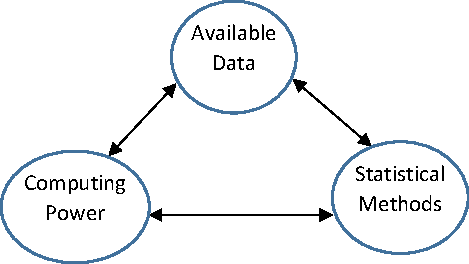
\includegraphics[width=.5\textwidth]{2_Background/figures/fig_Ml.pdf}
    \caption{The development cycle of Machine Learning.}
    \label{ch2:ml}
\end{figure}


 
 
 ML is more successful when it can be used to assist rather than replacing human experts; e.g. assist programmers to identify spam messages, assist engineers to optimize energy usage in homes, assist politicians to predict election outcomes, assist doctors to eradicate cancer, assist biologists to discover genetic sequences linked to the disease, assist policymakers to reduce the fraudulent credit card transactions, assist engineers to design self-driving cars, and more. Contrary and as part of their limits, computers are less flexible to extrapolate beyond the strict criteria learned. In addition, the ML algorithm is only as good as the data it learns from. If the input data does not contain an implicit context, the behavior of computers will be like humans; best guess.
 
The main purpose is to benefit from the computer experience to solve similar experiences in the future. Figure \ref{ch2:learning-process} shows the four interconnected parts of any learning process to answer the following questions: how the experience can be formed?, how learning can be transferred and understood by computers?     
 
 \begin{figure}[!ht]
    \centering
    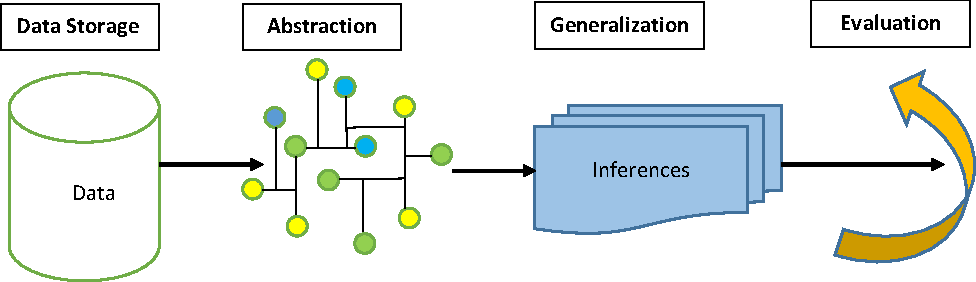
\includegraphics[width=.8\textwidth]{2_Background/figures/fig_learning-components.pdf}
    \caption{The four components of how to learn.}
    \label{ch2:learning-process}
\end{figure}
 
 \begin{enumerate}
     \item \textbf{Data Storage:} The main place to store data for the purpose of short-and long-term recall. Those data are represented as ones and zeros, with no meaning, on disks or random access memory (RAM). Memorizing the data can not be sufficient for the learning process, but it can be useful for reasoning; based on similar stored cases.  
     \item \textbf{Abstraction:} This phase is known as the knowledge representation or model training to assign meaning to stored data. The explicit description of the patterns within the data can be represented by different forms; e.g.(mathematical equations, interconnected diagrams like trees and graphs, logical IF-THEN rules, data clusters). For that, the original information can be summarized in a simple form with a discovery of unseen relations among data. No new data will be generated, only the original information can be seen from different perspectives of the representation form. 
     \item \textbf{Generalization:} The process of using the abstracted model for future actions on tasks which are similar to what has been seen before. Many discovered patterns can be noticed during the training phase, the most relevant pattern among data will be promoted as the most useful inference. For that, the model bias, which is the wrong in the prediction, usually will exist; as humans who are biased to take decisions based on past learned information. The uncorrelated bias (error) is a big benefit in ensemble learning, as we will discuss later.  
     \item \textbf{Evaluation:} Each model has its own bias which is inherited form the learned pattern. According to that, each model has its strengths and weaknesses. The final phase in learning, is to measure the model success in terms of bias to check if further training is needed. The evaluation is done to judge on the generalization capability for new, unseen, dataset. Finally, a model with a good performance during training, but with a poor evaluation, is said to be overfitted model. 
 \end{enumerate}
 
It is worth mentioning the ethics of machine learning and artificial intelligence. An automated algorithm working on emotionless devices can cause unintended consequences \cite{lantz2013}. The inference of those tools could be biased to racial, ethnic, and religious information in the dataset \cite{lantz2013}. For that and according to the application, that information should be blinded in data before training. It is important to have a clear understanding of; what we are doing?, why it is necessary to do it in an automatic way?, and how the implemented algorithm works?. In addition, some tools could help; like "FairML" \cite{adebayo2016} to know which algorithmic inputs could cause harm or bias. Finally, the user privacy and the behavior which is recorded through the web cookies should be respected. The availability of data does not give us the right to analyze it. 

In addition, the prediction result of an AI system could be explained in terms of the input data. The model-agnostic, post-hoc explainable technique, can be applied to any ML model regardless of its internal representation or process. Basically relies on the following sorted techniques according to their popularity: 

  \begin{itemize}[nosep]
      \item \textit{Explanation by simplification:} A new simplified model can be generated, keeping the similar performance score, while reducing the complexity. Popular techniques are local interpretable model-agnostic explanations (LIME \citep{ribeiro2016}), generic rule extraction methods (G-REX \citep{konig2008g}).
      \item \textit{Feature relevance explanation:} The opaque model can be explained by measuring the influence of each internal feature on the predicted output. Profitable contributions include: Shapley additive explanations (SHAP \citep{lundberg2017}) as a coherent method for describing the performance of any type of machine learning. As well, sensitivity analysis \citep{samek2017} to quantify the importance of the input variable based on partial derivative, but maybe sub-optimal for explaining AI and with several drawbacks \citep{montavon2018}. 
\item \textit{Visual explanation:} Portfolio of visualization techniques to explain the opaque model can be founded here \citep{cortez2011}. Furthermore, the use of individual conditional expectation plots (ICE \citep{goldstein2015}) for visualizing the estimated model by any supervised learning algorithm. 
  \end{itemize}